\section{Methods}
% \begin{center}
%     \begin{figure}
%     \makebox[\textwidth]{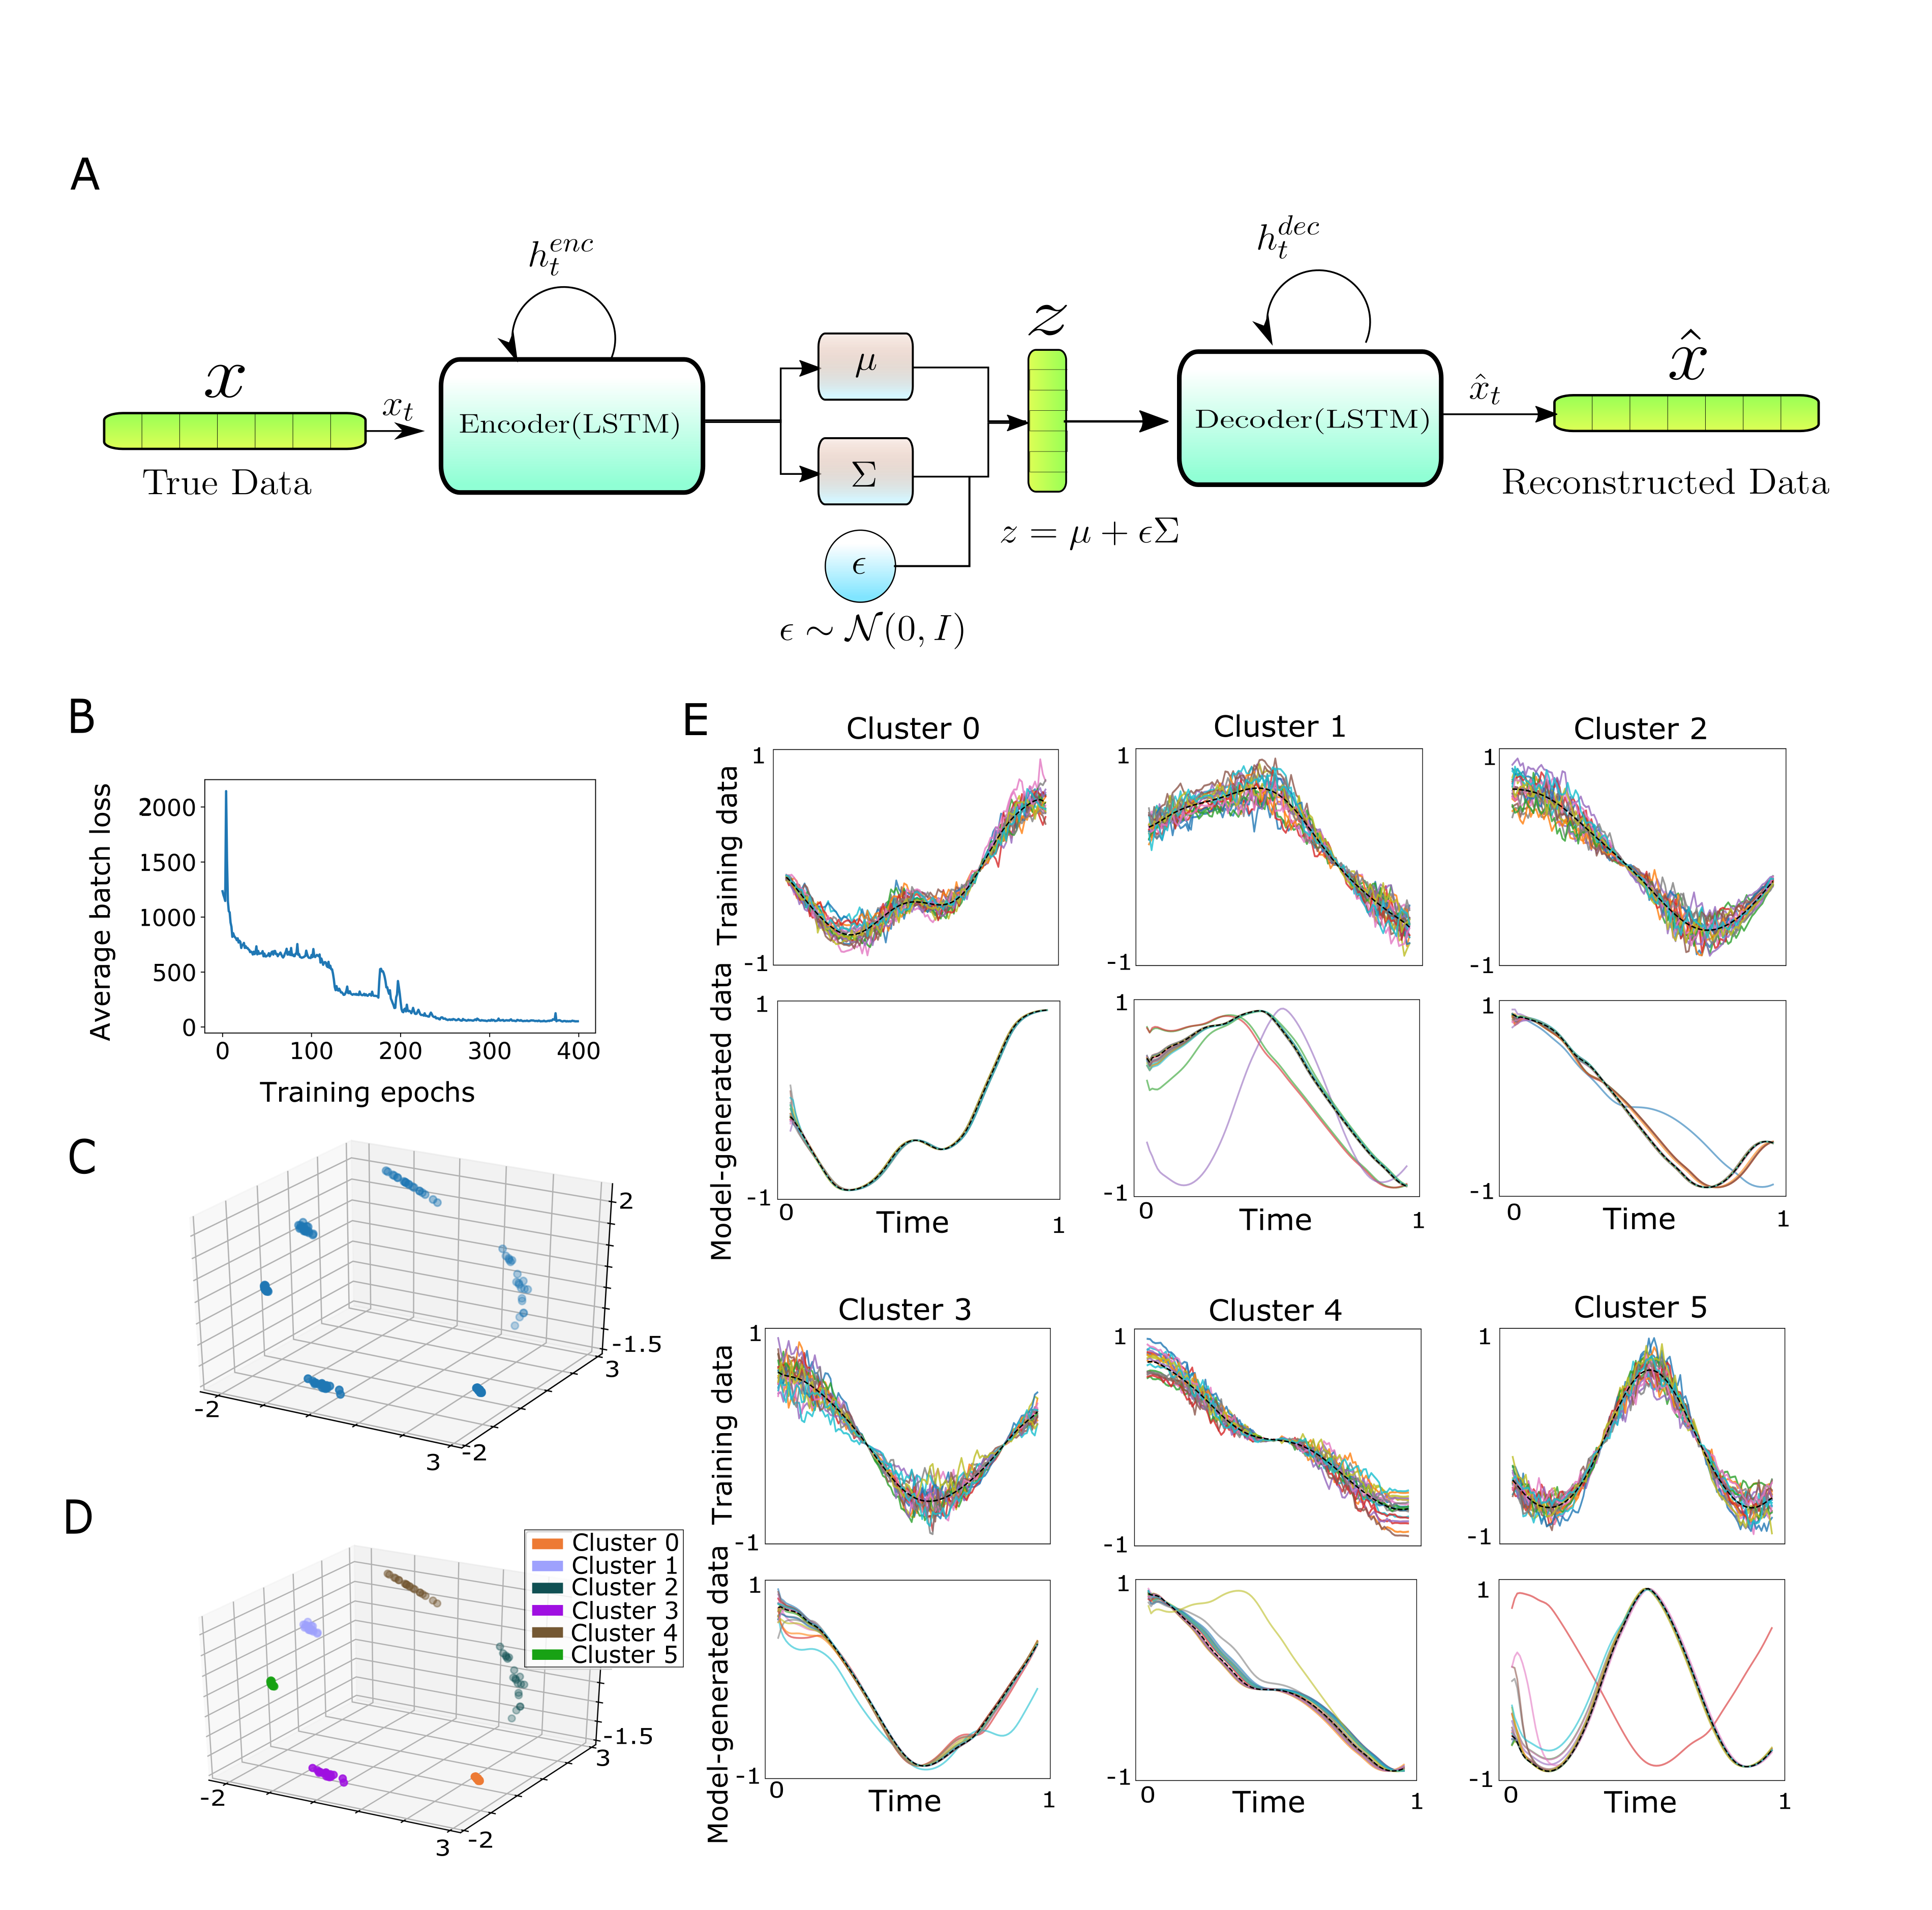
\includegraphics[width=0.8\paperwidth]{./pdna\_figs/fig1.png}}
%  % archetecture.png: 1149x508 px, 72dpi, 40.53x17.92 cm, bb=0 0 1149 508
%         \caption[Computational cost of training RVAgene]{\textbf{Training RVAgene is reasonably scalable on CPU and even more so using hardware acceleration through GPU.} ({\bf A}) Time cost of training RVAgene for 100 epochs for datasets with varying number of genes and time points on CPU and GPU. ({\bf B}) Maximum memory utilized during training of the model on CPU an GPU for the cases in (A), inset plot: comparison of max memory used compared to DPGP for varying number of genes.}
%   \label{fig:pdna1}
% \end{figure}
% \end{center}
\subsection{Position Weight Matrix (PWM)}
For the purposes of this study, a PWM is defined as an $N$ × 4 matrix,
where $N$ represents the length of the DNA of interest, and the four
positions correspond to the four DNA bases: adenine (A), cytosine (C),
guanine (G) and thymine (T). Each column in the PWM represents the
probabilities of the four bases occurring at that particular position.
\begin{align*}
Col_{PWM} &= [P_A, P_C, P_G, P_T]\\
P_A + P_C &+ P_G + P_T = 1
\end{align*}
\subsection{Ungapped Local Alignment}
Alignment of experimental PWMs to the corresponding co-crystal structure derived DNA is an important step for correctly annotating experimental protein-DNA structural data for model training and evaluation. This alignment needs to be ungapped and should prioritize alignment of higher IC columns from the PWM. Hence, we used an IC-weighted Pearson correlation coefficient (PCC) scoring scheme for the alignment, given by:

%%EQUATION
\begin{align}
ICWeightedPCC(Col_{PWM},Col_{DNA}) = PearsonR(Col_{PWM},Col_{DNA})\times \frac{IC(Col_{PWM})}{2}
\end{align}
where $PearsonR$ refers to a standard PCC, and $IC$ refers to the information content calculated for a probability simplex with a uniform background, in this context:
\begin{align}
IC([P_A,P_C,P_G,P_T]) = \sum\limits_{i\in[A,C,G,T]} \frac{log(P_i)}{log(0.25)}
\end{align}
%%EQUATION

%%ADD COMMENTS

\begin{pmialgorithm}[0.9\textwidth]{h!}{Ungapped Local Alignment}\vskip-2ex
        \label{algo:UngappedAlign}
        \begin{algorithmic}[1]
                \REQUIRE  $seq, pwm$ \COMMENT{Length X 4 arrays}
                \STATE  $max\_score \leftarrow -9999$
                \STATE  $opt\_i \leftarrow 0$
                \STATE  $opt\_j \leftarrow 0$
                \STATE  $opt\_k \leftarrow 0$
                \STATE  $l \leftarrow length(seq)$
                \STATE  $s \leftarrow length(pwm)$
                
                \FOR[]{$i=0,1,2,...,s-1$}
                \FOR[]{$k=0,1,2,...,s-i$}
                \FOR[]{$j=0,1,2,...,l-k$}
                \STATE  $score \leftarrow 0$
                
                \FOR[]{$col=0,1,2,...,k-1$}
                \STATE $col\_score \leftarrow ICWeightedPCC(pwm[i:i+k,:][col,:],$ \\$seq[j:j+k,:][col,:])$
                \STATE $score \leftarrow score + col\_score$
                \ENDFOR

                \IF[]{$score > max\_score$}
                \STATE $max\_score \leftarrow score + col\_score$
                \STATE $opt\_i \leftarrow i$
                \STATE $opt\_j \leftarrow j$
                \STATE $opt\_k \leftarrow k$
                \ENDIF
                
                \ENDFOR
                \ENDFOR
                \ENDFOR
                \RETURN $opt\_i, opt\_j, opt\_k, max\_score$
        \end{algorithmic}
\end{pmialgorithm}



\subsection{Representing DNA}
Our framework must consider several important factors for representing DNA. First, our model observes the structure of DNA in the input, but will predict a one-dimensional (1D) representation (a PWM). Thus, from an engineering perspective, it is beneficial to have the same number of features per base pair. Second, the input co-crystal structure derived DNA has a sequence; depending on the use case, we may or may not want our model to observe this sequence. Moreover, because experimental structural data are sparse, the co-crystal derived sequence has a strong potential for overfitting if observed by the model in the input. Therefore, in general, we want to symmetrize each base pair such that all sequence information is lost, but the global shape of the double helix is preserved. 

With these points in mind, we developed a coarse-grain symmetrized representation of DNA, where each base pair is represented by 11 points: two points for the phosphate moiety on each strand, two points for the sugar moiety, four points for the major groove, and three points for the minor groove. Major and minor groove points are placed symmetrically in the base-pair plane, so that they do not possess any particular base identity but roughly correspond to the major and minor groove chemical positions known \citep{Chiu2023} to be used for base readout. The phosphate moiety is represented by the coordinate of the phosphorus atom. The sugar moiety is represented by the average coordinate of all sugar heavy atoms. The three minor groove points divide the line segment connecting the two C1' atoms into four equal segments. The base-pair plane is determined by the triangle connecting the two C1' atoms and point O (average of atoms N1 and N9). Next, we move perpendicular (to the minor groove line segment) in this plane from either C1' for 3.75 \AA\  and expand the line segment by another 1.54 \AA\  in either direction. The line segment is divided into five equal segments to determine positions of the four major groove points. Additionally, the central two major groove points are shifted by an additional 1 \AA\ . This geometric construction is based solely on domain knowledge; no learning is employed to estimate any parameter. \hyperref[fig:pdnaS2]{Fig. S2a} shows a schematic representation of this process for an A-T base-pair. The only base atoms used for this process are N1 and N9, making it agnostic of base identity. \red{A step by step illustration of this process is provided in is \hyperref[fig:pdnaS32]{Fig. S32}}.

\hyperref[fig:pdnaS2]{Fig. S2b} shows an example transformation of a DNA structure to a symmetrized helix (sym-helix) using the described process. \hyperref[fig:pdnaS2]{Fig. S2c} shows one C-G base pair overlayed with sym-helix points computed for the corresponding base pair. As a result, the DNA structure is represented as $G^d = (V^d, X^d, N^d)$ .  $V^d$ represents coordinates of the sym-helix points, and $X^d$ represents point-level DNA features, which reflect a one-hot encoded annotation of the 11 positions in the symmetrized base-pair representation. If desired, we can reintroduce the DNA sequence (`DeepPBS with DNASeqInfo' model) by including base-pair-specific chemical group features for each point to $X^d$, as \citep{Chiu2023}. For each point , we also define an interaction vector $N^d_v$. These vectors act as reference directions in the base-pair frame. They are used to compute relative orientation-based features coupled with vectors $N^p$ on the protein graph (refer to Section 4). For the phosphate point, this vector is the average direction of the two double-bonded oxygens; for the sugar point, this vector is the direction of the C4'-C5' bond. For the seven major and minor groove points, these directions are determined by connecting each point to the centroid of the heptagon formed by these points. \hyperref[fig:pdnaS2]{Fig. S2e} shows the arrangement of these vectors on a sym-helix. These directions do not encode any base-specific information and only serve to inform the relative orientation of a sym-helix point in the context of binding. In addition, we include 14 DNA shape features \citep{Lavery2009, Lu2008, lavery1989defining} denoted as $X^s$, which are base-pair level features (\hyperref[fig:pdnaS2]{Fig. S2d}). These features are: buckle, shear, stretch, stagger, propeller twist, opening, shift, slide, rise, tilt, roll, helix-twist, major groove width, and minor groove width. 3DNAv2.3 \citep{Lu2008} and Curves5.3 \citep{Lavery2009, lavery1989defining} were used to calculate these values. Mean-padding was used to offset inter-base-pair features (shift, slide, rise, tilt, roll, helix-twist).

\subsection{Representing protein}

In our framework protein is viewed as a spatial graph $G^p = (V^p, X^p, E^p, N^p)$  where the
coordinates of the heavy atoms constitute the vertices $V^p$. For each vertex $v \in V^p$  we define
a set of features $X^p\_v$ which include one hot encoded atom type, solvent accessible surface area
of the atom, charge, radius, circular variance (7.5 $\AA$) and Atchley factors \citep{Atchley2005}. The edges $E^p$ of the protein
graph  are determined by the covalent bonds i.e. if  vertices $u$ and $v$ have
a covalent bond between them then $(u,v) \in E^p$. The edges are unordered. Lastly to encode
directionality of protein side chains we encode a unit vector $N^p\_v$ for each vertex $v$ computed by
averaging the directions of convalent bonds associated with each heavy atom. 

\subsection{DeepPBS architecture}
The architecture of DeepPBS is modular. First, the \textbf{ProteinEncoder} module applies spatial graph convolutions on the protein graph to aggregate neighborhood environment information for each protein heavy atom. Initially, a fully connected embedding layer is applied to $X_v^p \forall v \in G^p$, which expands the dimensionality of $X_v^p$ to 10 dimensions. Four layers of crystal graph convolutions (CGConv)\citep{Xie2018} are applied. The first two layers use only covalent bond edges, and the next two layers use distance-based edges with a 4\AA\  radius. The mathematical description of the message-passing scheme for CGConv is as follows:   
%%EQUATION
\begin{align}
X_v^p \leftarrow X_v^p + \big{(}\frac{1}{|\cN(v)|}\big{)}\sum\limits_{u\in\cN(v)}
\sigma(z_{uv}W_f + b_f)\odot g(z_{uv}W_s + b_s)
\end{align}
 
where $\cN(v)$ denotes the neighbors of $v \in V^p$ , and $z_{uv} = [X^p_v,X^p_u,e_{uv}]$ denotes the concatenation of target node features, source/neighboring node features, and edge features (here, the distance between u and v). In addition,  $\sigma$ denotes the sigmoid function, and $g$ denotes the softplus function. A Rectified Linear Unit (ReLU) \citep{Agarap2018} activation function is applied after each round of graph convolutions. This marks the end of the ProteinEncoder module.

The sym-helix point features $X_v^d$ are embedded into a 10-dimensional (10D) space using fully connected neural network layers and are used in the next module, the \textbf{Bipartite Geometric Network (BiNet)}. In this module, aggregated information on $G^p$ are pulled onto the sym-helix by performing geometry-aware bipartite convolutions. We use a modified version of point pair feature convolutions (PPFConv) \citep{Deng2018}, which we call a bipartite ResidualPPFConv. The message-passing update scheme associated with it is as follows: 
%%EQUATION
\begin{align}
X_v^d \leftarrow X_v^d + \gamma_\theta\bigg{(}\sum\limits_{u\in\cN(v),u\in V^p}h_\theta \big{(}
        x_u^p, ||d_{uv}||, \angle(N_v^d, d_{uv}), \angle(N_u^p,d_{uv}), \angle(N_v^d, N^p_u)
\big{)}
\bigg{)}
\end{align}

where $d_{uv}$ denotes the line segments connecting a sym-helix point $v$ and a protein heavy atom point $u$. $h_\theta$ is a transformation parametrized by fully connected neural networks. We set $\gamma_\theta$ to be the identity transformation. Four separate ResidualPPFConvs are applied for the major groove, minor groove, phosphate, and sugar points, respectively (from neighbors within 5 \AA), followed by ReLU activation. At this stage, we have aggregated all local chemical and geometric interaction contexts onto the sym-helix.

The final module is the \textbf{CNN-Predictor} module. We flatten the helix into a 1D base pair-level representation and apply a Multi Layered Perceptron (MLP) to reduce the dimensionality for each base-pair to 32. We concatenate precomputed helix shape features to aggregated base pair-level features. This step allows the network to make connections/correlate patterns between the aggregated information from BiNet and the global shape of the helix. We apply two rounds of 1D convolutions of filter size 3 with a stride of 1. We also apply relevant padding and set output feature size of 8, followed by ReLU activation, making the effective field of view five base-pairs. Next, we apply an MLP for each base-pair to generate logits for predicted base probabilities $([L_A,L_C,L_G,L_T])$ for corresponding base-pairs. We apply a SoftMax \citep{Bridle1990} activation to generate the output DNA base probabilities $([P_A,P_C,P_G,P_T])$. A global temperature parameter ($T_{glob}$) is learned for SoftMax through the training process. \hyperref[fig:pdnaS3]{Fig. S3} schematically describes the DeepPBS architecture.
\begin{align}
P_i = \frac{\frac{L_i}{e^{T_{glob}}}}{\sum\limits_{j\in[A,C,G,T]}\frac{L_j}{e^{T_{glob}}}} \forall i \in \{A,C,G,T\}
\end{align}
%%EQUATION
% 
% \begin{center}
%     \begin{figure}
%     \makebox[\textwidth]{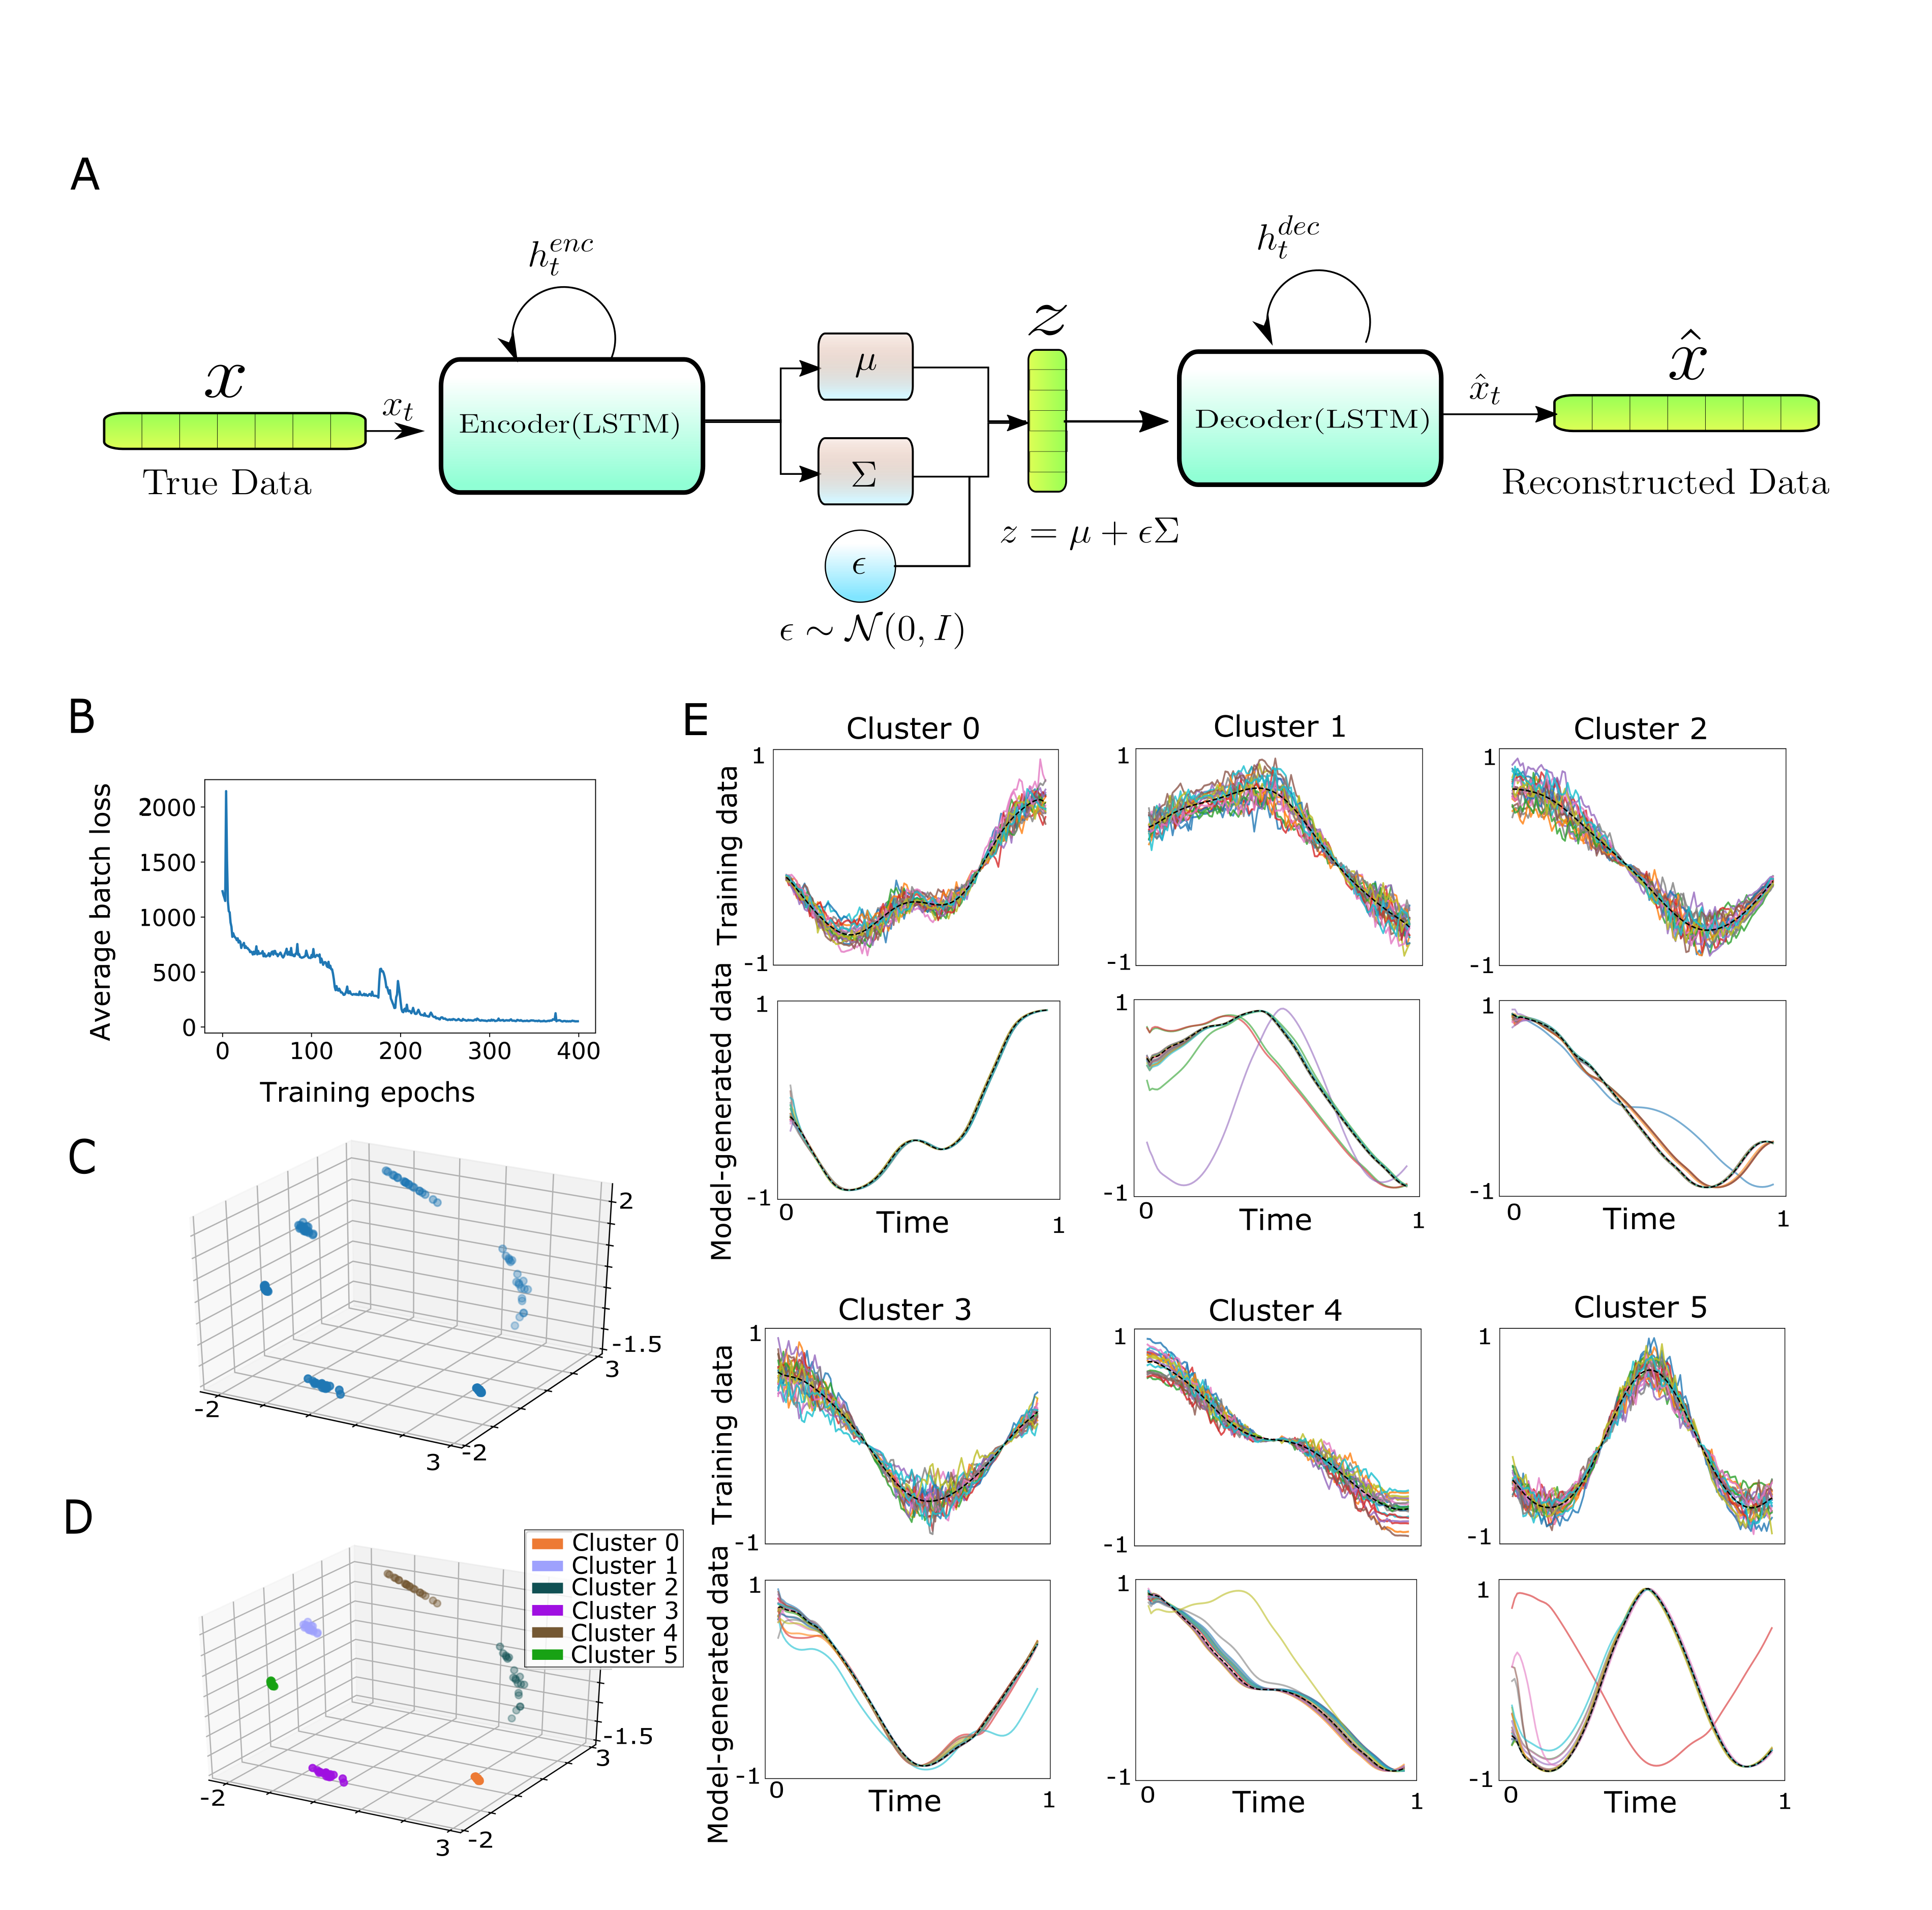
\includegraphics[width=0.8\paperwidth]{./pdna\_figs/fig2.png}}
%  % archetecture.png: 1149x508 px, 72dpi, 40.53x17.92 cm, bb=0 0 1149 508
%         \caption[Computational cost of training RVAgene]{\textbf{Training RVAgene is reasonably scalable on CPU and even more so using hardware acceleration through GPU.} ({\bf A}) Time cost of training RVAgene for 100 epochs for datasets with varying number of genes and time points on CPU and GPU. ({\bf B}) Maximum memory utilized during training of the model on CPU an GPU for the cases in (A), inset plot: comparison of max memory used compared to DPGP for varying number of genes.}
%   \label{fig:pdna2}
% \end{figure}
% \end{center}
\subsection{Training, cross-validation, and benchmarking}

Five models were trained for each of the four types: DeepPBS, DeepPBS GrooveReadout, DeepPBS ShapeReadout, and DeepPBS with DNA SeqInfo. Each model was trained on four folds of the constructed cross-validation set. Training was conducted for 50 epochs with early stopping on an NVIDIA RTX A4000 using an Adam \citep{Kingma2017} optimizer, with a learning rate of 0.001 and weight decay of 0.0001. Hyperparameters were selected based on domain knowledge and training curves. For every datapoint, two forward passes were made to account for reverse complement predictions for both strand directions (with relevant index transformations for input; refer to Data/Code Availability). Outputs were concatenated, and MAE loss was calculated with ground truth (corresponding PWM and its reverse complement concatenated). Predictions were made on the corresponding fifth/validation fold with each model to gather predictions for all datapoints in the 5-fold dataset. These predictions were used to report metrics in \hyperref[fig:pdnaS5]{Fig. S5a-c}. 

For benchmarking purposes, ensemble averaged (of the five trained cross-validation models) predictions are used \blue{Fig. 2.3a-d}. The ensemble is also used for results presented in \blue{Fig. 2.4, 2.5, 2.6}, and \blue{Fig. S5b,d, S6, S7, S8, and S9}. All core DeepPBS code was written in python3.9+ with various pythonic dependencies (full list available at \href{https://github.com/timkartar/DeepPBS}{GitHub}). Packages used for geometric deep learning are pytorch1.12+ and torch-geometric (pyg v2.0+).

\subsection{Performance metrics}

Performance metrics used in this chapter are MAE and RMSE, defined as 
%%EQUATION
\begin{align*}
\text{MAE}(Y, Y^{pred}) &= \frac{1}{N} 
\sum\limits_{i\in\{0,..,N-1\}} \sum\limits_{b\in\{A,C,G,T\}} |Y_{ib} - Y_{ib}^{pred}|\\
\text{RMSE}(Y, Y^{pred}) &= \sqrt{\frac{1}{N} \sum\limits_{i\in\{0,..,N-1\}} \sum\limits_{b\in\{A,C,G,T\}} (Y_{ib} - Y_{ib}^{pred})^2}
\end{align*}

$N$ refers to the number of columns in the PWMs being compared. Both metrics follow ‘the lower the better’ principle. They are not independent but have different properties. 

\subsection{Additional discussion on behavior of metrics}

To get a better perspective of the behavior of MAE metric, we demonstrated of how the MAE metric behaves for various different target PWM columns and possible predictions (\hyperref[fig:pdnaS10]{Fig. S10a}). The predictions are of three forms, based on interpolated values of a variable $x\in[0,1]$. They are as follows: %%EQUATION
\begin{align}
[1-x,0,x,0], [x, \frac{1-x}{3}, \frac{1-x}{3}, \frac{1-x}{3}], [\frac{1-x}{3}, \frac{1-x}{3}, \frac{1-x}{3}, x]
\end{align}
. These demonstrations, although they do not form an exhaustive set, but gives an idea of the behavior of the MAE metric. Based on these plots and taking into account the inherent performance limit computed for this metric, we can consider values less than 0.8 to be of reasonable agreement and below 0.6 to be in good agreement. Although, we do note that these values should not be set in stone as the problem in question is a regression problem as opposed to binary classification.

Some further thoughts on this matter: In theory, the uniform prediction [0.25, 0.25, 0.25, 0.25] can be regarded as a bad prediction, because a naive model can always predict such a value. This prediction will perform well for highly non-specific binders (e.g., cases like \hyperref[fig:pdnaS8]{Fig. S8}) but will fail for highly specific binders. However, the one-hot prediction [1,0,0,0] can also be a naive (bad) prediction for this problem setting. It is the case when the sequence present in the co-crystal structure itself is the output, e.g., for the sequence ACG: [[1,0,0,0],[0,1,0,0],[0,0,1,0]]. For experimentally determined structures, this prediction will generally perform well, especially for highly specific binders, but will fail for nonspecific binders. Ultimately, we wanted to create a general model that can handle specific binders and non-specific binders. So, we need a target metric to strike a balance between both scenarios. Therefore, in our opinion, looking at the predictive performances in context of the alignment scores of the co-crystal structure derived sequence with the target PWM gives a clearer picture. This has now been added (for the benchmark set) to the manuscript as \hyperref[fig:pdnaS10]{Fig. S10b}.

We choose a continuous distance metrics like MAE over statistical measures like PCC (Pearson R) or SCC (Spearman R) because they are not very robust with only four (linearly dependent) points (well-known result in the statistics community \citep{Bonett2000, McIntyre1938}. In our observation, SCC can only take a few discrete values in this scenario and can sharply change for a very small change of values that change the rank order. The PCC metric, although it takes continuous values, is affected by similar non-intuitive situations. This is easy to demonstrate by considering the following three slightly altered predictions:
\\
PCC([0.5,0.5,0,0], \textbf{[0.25,0.25,0.25,0.25]}) = Undefined\\
PCC([0.5,0.5,0,0], \textbf{[0.23,0.24,0.26,0.27]}) = -0.9487\\
PCC([0.5,0.5,0,0], \textbf{[0.27,0.26,0.24,0.23]}) = 0.9487\\
(calculated using scipy.stats.pearsonr() function)

Intuitively, all three predictions are of similar caliber. However, the PCC metric paints a dramatically different picture. MAE on the other hand produces values of 1, 1.06 and 0.94. This is much more nuanced and intuitive. We can also easily construct other non-intuitive situations for PCC. For example, if the target is [0.1,0.2,0.3,0.4], any monotonically increasing prediction will have a high PCC value.

PCC([0.1,0.2,0.3,0.4], \textbf{[0.001,0.002,0.003,0.994]}) = 0.776

This gives the impression that this prediction is quite good, while in reality, it is almost just a one-hot prediction. MAE on the other hand produces a value of 1.187 which depicts a bad prediction.

\subsection{Additional details associated with application of DeepPBS on predicted structures}
%% CHECK LINKS

\textbf{Running rCLAMPS}: We ran the rCLAMPS model with default parameters provided by the model’s authors according to instructions provided through their GitHub.
\\
\textbf{Running RoseTTAfoldNA (RFNA)}: We ran the RFNA model with default options and model weights (version: April 13, 2023 v0.2) as provided by the authors through their GitHub.
\\
\textbf{Trimming unstructured regions from full-length homeodomain (HD) sequences}: For the analysis in \hyperref[fig:pdna3]{Fig. 2.4e-i}, full-length HD sequences were first trimmed to remove unstructured regions, while retaining the main Homeobox domain of interest (rCLAMPS also applies the same process in its pre-processing). This step was achieved by HMMERv3.4 \citep{Finn2011} using the ‘homeobox.hmm’ file provided by the rCLAMPS repository. 
\\
\textbf{MM-PBSA vacuum energy calculation}: For each PDB file, we generated a topology file and a run-parameter file using Gromacs 2020.3 to define the force fields amber14sb for protein and parmbsc1 for DNA. These files were used as input for g$\_$mmpbsa to calculate the potential energy in a vacuum. The dielectric constant of the solute was set to 8. 
\\
\textbf{Dataset}: We obtained UniProt protein sequences for three different families, bZIP (homodimers), bHLH (homodimers), and homeodomain (HD) (heterodimers excluded), for cases with a corresponding unique JASPAR entry and no experimental structure for the complex. RFNA predictions that could be successfully processed by DeepPBS pre-processing steps were fed into DeepPBS for specificity prediction (n=49 for bHLH, n=50 for bZIP, n=236 for HD family members).
\\
\textbf{Choice of initial guess (IG) DNA}: The IG DNA for the bHLH family was chosen as ‘GCGCACCACGTGGTGCGC’, which has a center E-box motif (‘CACGTG’) that is known \citep{demartin2021} to be a bHLH family target. The IG DNA for the bZIP family was chosen as ‘GCGCTGATGTCAGCGC’ (based on human CREB1 motif MA0018.4). The IG DNA for the HD family was chosen as ‘GCGTGTAAATGAATTACATGT’, based on DNA from PDB ID 1APL. 
\\
\textbf{Details on metric calculation for \hyperref[fig:pdna3]{Fig. 2.4d}}: We calculated MAE (best full overlap) for predictions in \hyperref[fig:pdna3]{Fig. 2.4d} against corresponding JASPAR annotations. As a baseline (apart from random predictions drawn from uniform), we calculated the MAE (best full overlap) for the one-hot PWM determined by the IG DNA against the corresponding JASPAR annotation. For the bHLH and HD families, the IG DNA was closer to experimental data than to random baseline (\hyperref[fig:pdna3]{Fig. 2.4d}).
\\
\textbf{pLDDT score}: (RFNA-predicted LDDT (Local Distance Difference Test) score \citep{Mariani2013}). The LDDT score measures the similarity between a predicted and reference structure. When predicting a complex structure, RFNA predicts an LDDT score (pLDDT). These pLDDT scores were shown \citep{baek2024na} to be well correlated with the true LDDT of RFNA predictions. Thus, the pLDDT can be taken as a measure of quality of a complex generated by RFNA.
\\
\textbf{Comparison of DeepPBS and rCLAMPS}: There are several qualitative advantages to the DeepPBS approach. First, rCLAMPS uses structural mapping for HD-DNA binding to predict specificity for a given HD sequence. This structural mapping leads to a specificity output of exactly six 6 base pairs (bp). DeepPBS is functionally not limited to only predicting a 6-base pair core and can predict preferences in the flanks (\hyperref[fig:pdna3]{Fig. 2.4e}). Second, rCLAMPS is restricted to predicting monomer preferences (although HD proteins can often bind as dimers; see, e.g., \hyperref[fig:pdnaS6]{Fig. S6a}). In contrast, DeepPBS is able to handle biological assemblies. Third, DeepPBS is not limited to a specific family. For quantitative comparison, we compare the aspects that are achievable by rCLAMPS, namely, 6mer specificity predictions for monomer HD proteins.
\\
\textbf{Metric computation for comparison with rCLAMPS}: We ran rCLAMPS (github commit version 32a94edb65e87c6d038823dc34c4bcf6e1071b7b) on the set of monomer HD proteins (with unavailable complex structure, i.e. not part of RFNA or DeepPBS training). We computed the MAE (best overlap) values for rCLAMPS predictions against the corresponding JASPAR entry of experimental data, and compared these values to the MAE values of the best 6-mer overlap for DeepPBS predictions. In this case, for each datapoint, one of round 4-7 prediction was chosen. This choice was based on maximizing corresponding protein-DNA contact count (5 \AA cutoff) of input RFNA predicted structure. 
\\
\textbf{Folding benchmark set datapoints with RFNA}: We refolded all the benchmark set datapoints with RFNA, for results presented in \hyperref[fig:pdna3]{Fig. 2.4g}. 108/130 RFNA predictions produced pre-processable results. Out of them a few of were not able to place the protein near the DNA helix properly. So, we filtered an atom-to-atom contact count (within 5 \AA) of greater than 500 contacts between protein and DNA to filter this set producing a set of size 98. The high confidence set among these are taken as predictions for which the RFNA pLDDT was greater that 0.9.

\subsection{Molecular Dynamics (MD) simulation of Exd-Scr–DNA system}
We conducted MD simulations on the Drosophila Extradenticle (Exd)-Sex combs reduced (Scr) system, with the dimer bound to its target DNA, using the co-crystal structure (PDB ID: 2R5Z). AlphaFold2 predictions of the proteins were aligned to the PDB structure to create an initial structure of the simulation. This process aided in filling in the missing linker residues in the biological assembly. The simulation was executed using the Gromacs \citep{Abraham2015} 2020.3 software package. Protein interactions were modeled with the amber14sb \citep{Maier2015} force field, and DNA interactions were modeled with the parmbsc1 \citep{Ivani2016} force field. The pdb2gmx program from Gromacs was used to generate topological information for the simulation. The -his flag was used to protonate both N$\delta$ and N$\epsilon$ atoms of the His-12 residue for the system with protonated His-12. All complexes were solvated using the explicit TIP3P water model. The negative net charge of the Exd-Hox-DNA complex was neutralized by adding positively charged Na+ counterions, along with negatively charged Cl- counterions, to reach a final NaCl concentration of 150 mM that approximates the physiological concentration. The GROMACS 2020.3 genion program was used to place these counterions throughout the box. 
\par
The protein-DNA complex was energy-minimized with steep descent energy minimization for 2,000 steps to relax the structure and remove any steric clashes. Next, we performed three rounds of gradual NVT (constant Number of particles, Volume, and Temperature) equilibration for 10 ps to slowly heat the prepared system to 300K and 1 round of NPT (constant Number of particles, Pressure, and Temperature) to equilibrate the pressure of the system to 1 bar for 700ps. These equilibration rounds were used to adjust the whole system to biological conditions before starting the production simulation. The production simulation for the system was run for 300 ns in the isobaric–isothermal ensemble, where the pressure was maintained at 1 bar and temperature at 300K. The integration time step of 2 fs was used for all calculations. The Verlet cutoff scheme was used for all calculations. Long-range electrostatic interactions were computed using the Particle Mesh Ewald method \citep{Darden1993} from the GROMACSv2020.3 package, with a 12\AA cutoff. Nonbonded van der Waals interactions were calculated with a 12\AA cutoff. The LINCS \citep{Hess1997} algorithm from the GRPMACSv2020.3 package, was employed to constrain all bonds.The MD simulation trajectories were generated as part of a recent study exploring effects of minor groove linker histidine protonation \citep{Jiang2023}.
\\
\subsection{Measures ensuring prevention of overfitting to protein sequences}
We took several steps to prevent the model to be overfit on protein sequences. The cross-validation fold creation script (see Code Availability) took care to keep members of the same cluster in the same fold (except a handful ($<4\%$) got split randomly to keep the fold sizes same). Full description of these splits is available (see Data Availability) and the code for this process is available (see Code Availability). In addition, no more than five samples were chosen per cluster into a fold. This ensures prevention of over representation. Furthermore, the input to DeepPBS is purely structural and physico-chemical, and does not contain the sequence representation. These structures may demonstrate different spatial conformations interacting with potentially different DNA sequence/shape and randomly picked target PWM from JASPAR or HOCOMOCO. These guardrails in architecture and all of these variations, even for similar protein sequences, makes the model less prone to overfit on protein sequences. 
\\
\subsection{Bipartite edge perturbation and protein heavy atom importance score calculation}
Supplementary \hyperref[fig:pdnaS4]{Fig. S4} schematically describes the bipartite edge perturbation process for calculating protein heavy atom (say, atom a) importance scores. Briefly, the prediction is calculated twice: once (say, $Y_a$) while considering edges corresponding to the protein heavy atoms, and again (say, $Y_{\sim a}$) while masking the same edges. This process results in differences in predictions, which can be calculated using the mean absolute difference measure. On their own, these values may not be meaningful, but they can be normalized to the 0–1 range by dividing by the maximum value within a structure. The normalized values, RI scores, signify how much the specificity prediction is influenced by interactions made by the corresponding heavy atom. Depending on the downstream use, RI scores can be aggregated at the residue level using either the average, max or sum aggregations. Mathematically,
\begin{align} 
RI_\alpha = 
\frac{\text{MAE}(Y_a,Y_{\sim a})}
{max_{\{b\in all\ atoms\}}\text{MAE}(Y_b,Y_{\sim b})}
\end{align}
\par
Computationally, this process is like measuring the effect of a deactivating mutation, which is why we hypothesized that, at a residue level, these scores could correlate with alanine scanning mutagenesis data. For comparison with alanine scanning mutagenesis experiments (\hyperref[fig:pdna4]{Fig. 2.5h}) at a residue level, the log sum aggregated importance score was calculated. For each atom a of a residue r in the protein–DNA interface, let the calculated RI be RIa. Then, this value is calculated as
\begin{center}
LogSum aggregated residue importance($r$) = $log_2(1 + \sum\limits_{a\in r}RI_\alpha)$ %%EQUATION
\end{center}
Structure visualizations presented were produced using PyMOL2.5 \citep{pymol}.

\subsection{Description of competitor assay for quantifying designed proteins’ binding specificity}

Glasscock et al. \citep{Glasscock2023} used a yeast display assay to quantify binding of their designed proteins. The proteins were expressed by integrating the corresponding synthetic oligonucleotide to a yeast surface expression vector. Yeast cells expressing designed proteins on their surface were labeled with biotinylated dsDNA targets, streptavidin–phycoerythrin and anti-c-Myc fluorescein isothiocyanate in a 96-well plate format, after which a binding signal was quantified on an Attune NxT flow cytometer. Excess addition of a competitor nonfluorescent target DNA reduces this binding signal. Thus, scanning single mutations for each position was possible through the competitor producing the data shown in \hyperref[fig:pdna5]{Fig. 2.6d,h,l,p}.
\\
\subsection{DeepPBS webserver}
DeepPBS is available as a webserver at https://deeppbs.usc.edu. The webserver provides the functionality of the DeepPBS method of predicting a PWM on the basis of the structure of a protein–DNA complex. The structure can be uploaded as a PDB or macromolecular crystallographic information file. The webserver provides a documentation for users.
